\clearpage

\subsection{Scan Brats18\_2013\_17\_1 layer 1}
In this section we discuss the results when applying Hausdorff Distance Masks to the first extracted layer from the scan "Brats18\_2013\_17\_1".

\subsubsection{Results T1}

\begin{figure}[H]
    \centering
    \begin{subfigure}[t]{.4\textwidth}
        \centering
        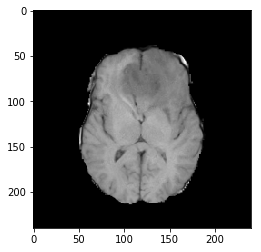
\includegraphics[width=\linewidth]{chapters/06_hdm/c_Brats18_2013_17_1_L1/41.png}
        \caption{T1 modality slice}
    \end{subfigure}\hspace{1cm}%
    \begin{subfigure}[t]{.4\textwidth}
        \centering
        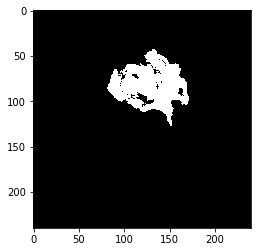
\includegraphics[width=\linewidth]{chapters/06_hdm/c_Brats18_2013_17_1_L1/40.png}
        \caption{Tumor ground truth}
    \end{subfigure}
    \begin{subfigure}[t]{.45\textwidth}
        \centering
        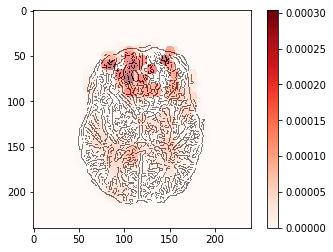
\includegraphics[width=\linewidth]{chapters/06_hdm/c_Brats18_2013_17_1_L1/43.png}
        \caption{Regions where the applied masks reduce the accuracy of the segmentation}
    \end{subfigure}\hspace{1cm}%
    \begin{subfigure}[t]{.45\textwidth}
        \centering
        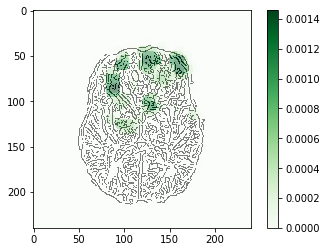
\includegraphics[width=\linewidth]{chapters/06_hdm/c_Brats18_2013_17_1_L1/44.png}
        \caption{Regions where the applied masks increase the accuracy of the segmentation}
    \end{subfigure}
    \caption{Modality T1 analyzed with Hausdorff Distance Masks.}
    \label{brats_201317_t1}
\end{figure}

\begin{figure}[H]
    \centering
    \begin{subfigure}[t]{.4\textwidth}
        \centering
        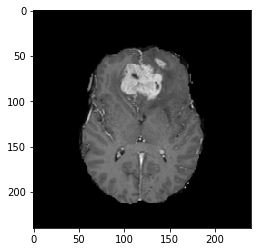
\includegraphics[width=\linewidth]{chapters/06_hdm/c_Brats18_2013_17_1_L1/46.png}
        \caption{T1 contrast enhanced modality slice}
    \end{subfigure}\hspace{1cm}%
    \begin{subfigure}[t]{.4\textwidth}
        \centering
        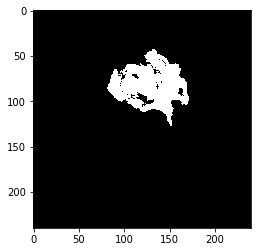
\includegraphics[width=\linewidth]{chapters/06_hdm/c_Brats18_2013_17_1_L1/45.png}
        \caption{Tumor ground truth}
    \end{subfigure}
    \begin{subfigure}[t]{.45\textwidth}
        \centering
        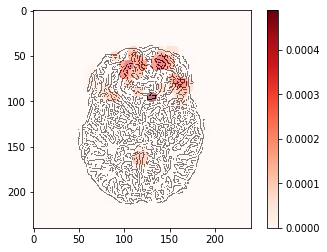
\includegraphics[width=\linewidth]{chapters/06_hdm/c_Brats18_2013_17_1_L1/48.png}
        \caption{Regions where the applied masks reduce the accuracy of the segmentation}
    \end{subfigure}\hspace{1cm}%
    \begin{subfigure}[t]{.45\textwidth}
        \centering
        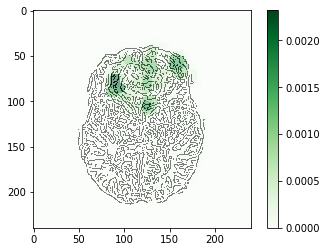
\includegraphics[width=\linewidth]{chapters/06_hdm/c_Brats18_2013_17_1_L1/49.png}
        \caption{Regions where the applied masks increase the accuracy of the segmentation}
    \end{subfigure}
    \caption{Modality T1 contrast enhanced analyzed with Hausdorff Distance Masks.}
    \label{brats_201317_t1ce}
\end{figure}

\begin{figure}[H]
    \centering
    \begin{subfigure}[t]{.4\textwidth}
        \centering
        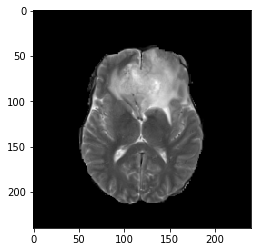
\includegraphics[width=\linewidth]{chapters/06_hdm/c_Brats18_2013_17_1_L1/51.png}
        \caption{T2 modality slice}
    \end{subfigure}\hspace{1cm}%
    \begin{subfigure}[t]{.4\textwidth}
        \centering
        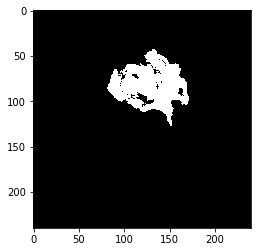
\includegraphics[width=\linewidth]{chapters/06_hdm/c_Brats18_2013_17_1_L1/50.png}
        \caption{Tumor ground truth}
    \end{subfigure}
    \begin{subfigure}[t]{.45\textwidth}
        \centering
        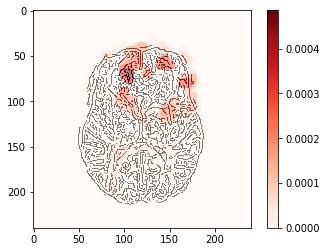
\includegraphics[width=\linewidth]{chapters/06_hdm/c_Brats18_2013_17_1_L1/53.png}
        \caption{Regions where the applied masks reduce the accuracy of the segmentation}
    \end{subfigure}\hspace{1cm}%
    \begin{subfigure}[t]{.45\textwidth}
        \centering
        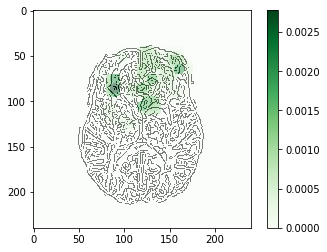
\includegraphics[width=\linewidth]{chapters/06_hdm/c_Brats18_2013_17_1_L1/54.png}
        \caption{Regions where the applied masks increase the accuracy of the segmentation}
    \end{subfigure}
    \caption{Modality T2 analyzed with Hausdorff Distance Masks. }
    \label{brats_201317_t2}
\end{figure}

\begin{figure}[H]
    \centering
    \begin{subfigure}[t]{.4\textwidth}
        \centering
        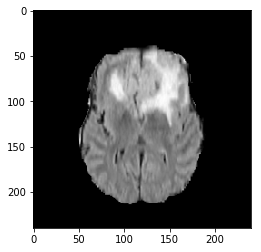
\includegraphics[width=\linewidth]{chapters/06_hdm/c_Brats18_2013_17_1_L1/56.png}
        \caption{FLAIR modality slice}
    \end{subfigure}\hspace{1cm}%
    \begin{subfigure}[t]{.4\textwidth}
        \centering
        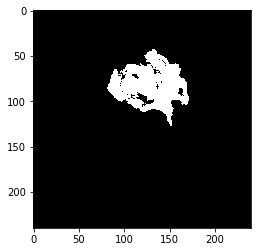
\includegraphics[width=\linewidth]{chapters/06_hdm/c_Brats18_2013_17_1_L1/55.png}
        \caption{Tumor ground truth}
    \end{subfigure}
    \begin{subfigure}[t]{.45\textwidth}
        \centering
        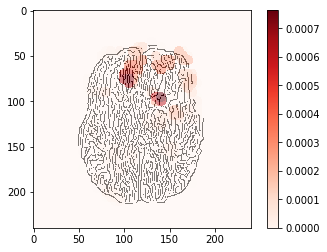
\includegraphics[width=\linewidth]{chapters/06_hdm/c_Brats18_2013_17_1_L1/58.png}
        \caption{Regions where the applied masks reduce the accuracy of the segmentation}
    \end{subfigure}\hspace{1cm}%
    \begin{subfigure}[t]{.45\textwidth}
        \centering
        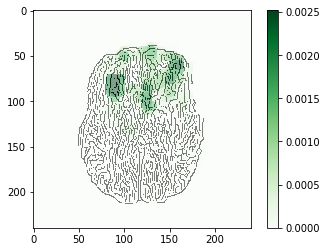
\includegraphics[width=\linewidth]{chapters/06_hdm/c_Brats18_2013_17_1_L1/59.png}
        \caption{Regions where the applied masks increase the accuracy of the segmentation}
    \end{subfigure}
    \caption{Modality FLAIR analyzed with Hausdorff Distance Masks.}
    \label{brats_201317_flair}
\end{figure}

\subsubsection{Discussion}
Figures \ref{brats_201317_t1}, \ref{brats_201317_t1ce}, \ref{brats_201317_t2} and \ref{brats_201317_flair} show HDM results applied on all four modalities. In comparison to the analyzed scans in the previous section, these visualization show that the neural network mainly looks at the border of the tumor, with the exception of the T1 modality. To generate a segmentation, the borders of the tumor are very important, and it seems the neural network successfully learns this fact.